In this section, we present the {\em RambutanAcc's} task dependency graph representation (or task graph for short) followed by the execution model governing the execution of a task graph program.
Our design goal is to keep the programming API as simple as possible.


\subsection{Task and Data Spaces}
Each {\em RambutanAcc} application works on a directed acyclic graph (DAG) in which vertices are {\em tasks} (see Fig.~\ref{fig:taskGraph}).
A {\em task} is a sequence of statements.
{\em Tasks} are atomic, meaning that when a task is scheduled it runs to completion.
{\em Tasks} are created and destroyed at runtime.
{\em RambutanAcc} separates the task space from data space.
The programmer defines an ownership function to map tasks to partitions of the data space.
Each data partition is associated with an attribute called {\em locale}, which indicates the location of the data (e.g. in GPU's memory).
Task and data do not have to reside in the same physical place, and it is the responsibility of the runtime to move required data to tasks.
The programmer specifies task's inputs and outputs, which are data partitions.
We next describe the full process of defining a task.


\begin{figure}[htb]
\centering
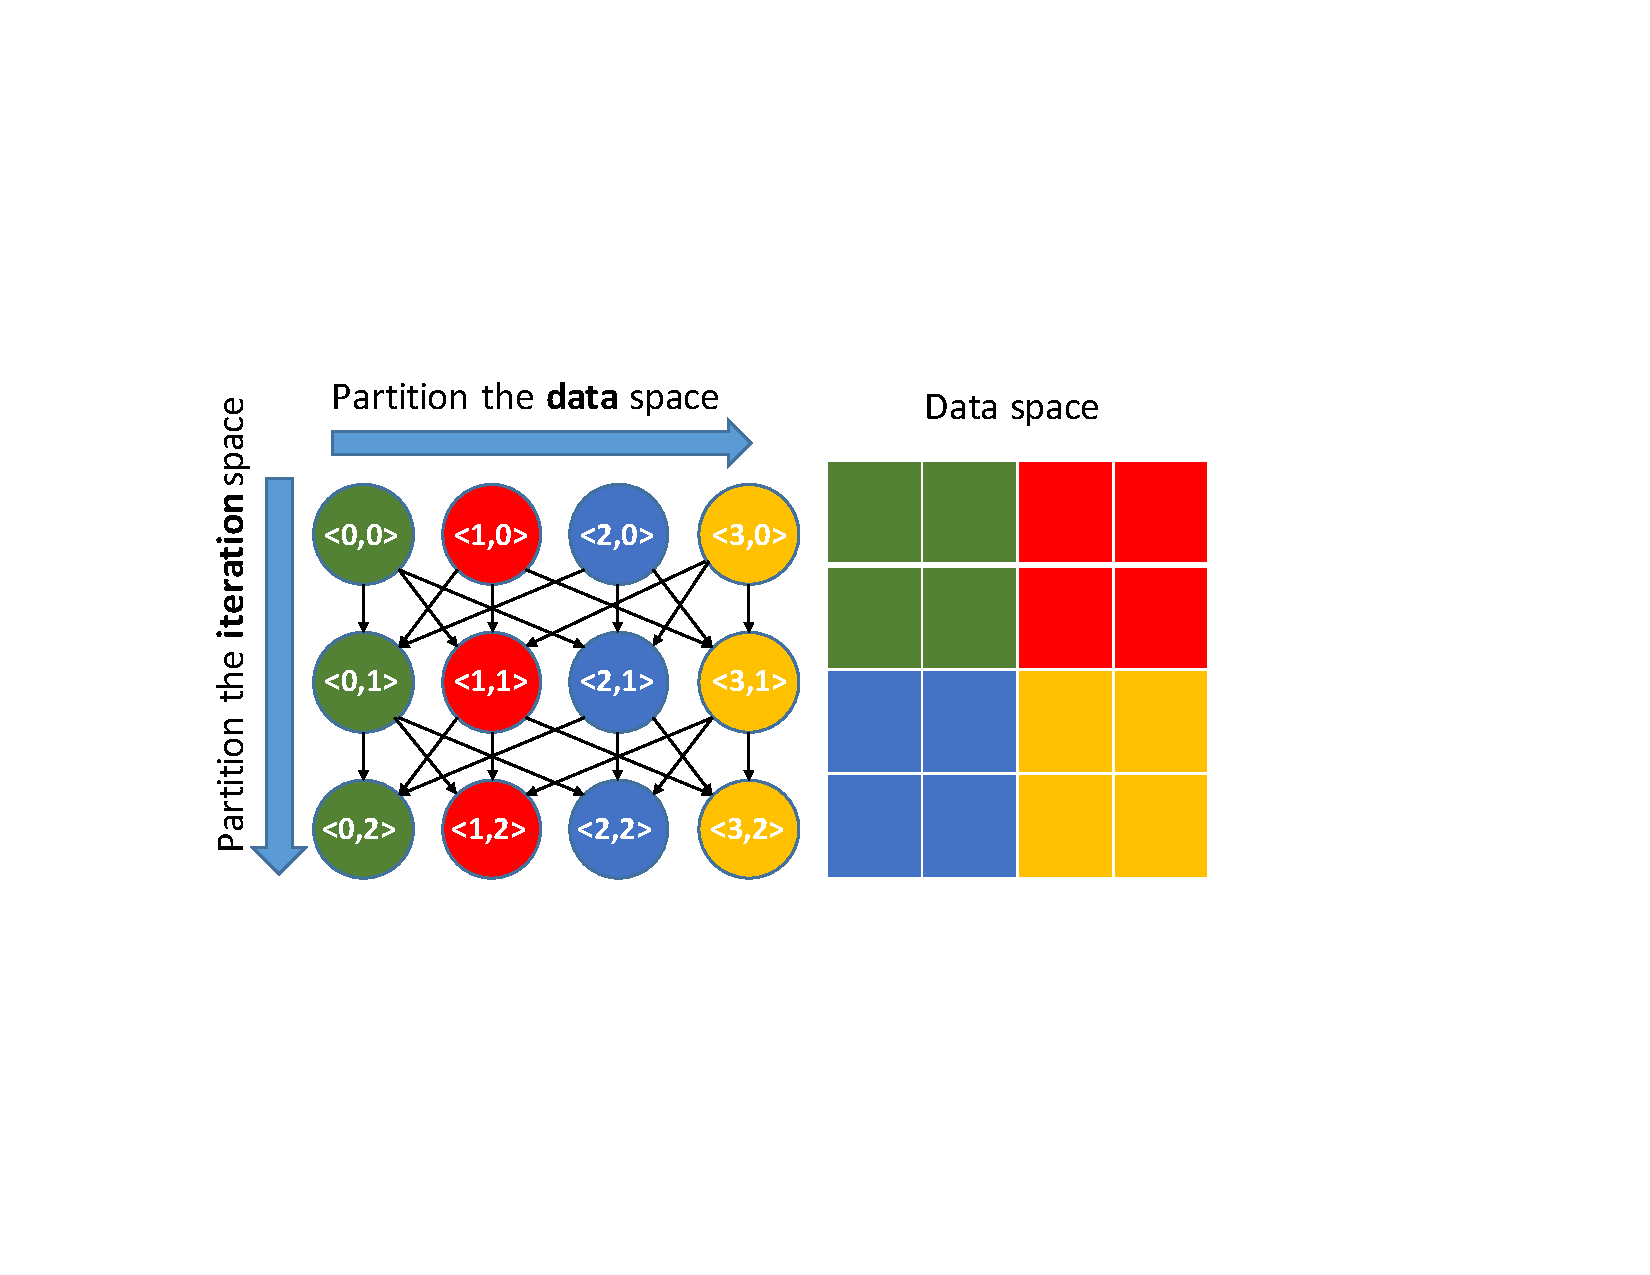
\includegraphics[width=.47\textwidth]{figures/taskGraph.pdf}
\caption{A directed acyclic graph for an iterative solver in two dimensions. The graph partitions the data space and the iteration space. Data space is divided into four partitions, and the color represents the ownership mapping function (tasks to data partitions). Task identifier is a pair of data partition ID and iteration number. Arrows among tasks of different colors represent the data dependencies on ghost cells. Arrows among tasks of the same color represent the task creation order.} 
%Tasks are fireable as soon as data dependencies are satisfied.}
\label{fig:taskGraph}
\end{figure}


\subsection{Defining a task}
For tasks running completely on the host, defining a task includes the specification of inputs and outputs, statements that the task will execute, and new task creation requests.
For tasks running on the accelerator, the programmer has two options for the statement specification phase: (i) each task has some code running on the host to launch the kernel on the accelerator (ii) the runtime directly schedules tasks on accelerator.
In both cases, the runtime handles the communication to make sure that the task is scheduled only when all inputs are available.
%However, in the former case, each task can launch multiple kernels.
In the former case, the programmer has to prepare all arguments needed for the kernel launch and all the required synchronization.
In the latter case, the runtime is responsible for offloading the code and argument information to the accelerator.
With this option, the task can invoke other functions without any special support from hardware (e.g. dynamic parallelism support from CUDA).


\subsection{Execution model}
Among tasks, there are ones that can run without any input from other tasks.
These tasks are called {\em roots}.
In the task graph program described in Fig.~\ref{fig:taskGraph}, tasks ($<$0, 0$>$, $<$1, 0$>$, $<$2, 0$>$, and $<$3, 0$>$ are roots since at the first iteration no nearest neighbor update is required.
Once a {\em root} task finishes its execution, output can be produced.
Now the task notifies the runtime about the availability of the data so the runtime can create new tasks (even remote tasks) and fetch the just produced output data to their locations.
As soon as the data required by a new task have been fetched, that task can become runnable.
Runnable tasks will be scheduled to execute by {\em RambutanAcc} {\em workers}, which can be CPU cores, accelerator, or a portion of the accelerator.
The runtime scheduler periodically checks the availability of {\em workers} to schedule tasks. 
A {\em worker} can be configured with a task buffer having more than one slot so that the scheduler can assign tasks even when the {\em worker} is busy (pre-scheduled). 
This capability allows tasks to be offloaded to {\em workers} on the accelerator at zero cost, since the time to move function arguments from host to accelerator can be overlapped with the execution of another task.

A notable concern when programming on accelerators is that the DRAM capacity on accelerator is often modest compared to host DRAM.
If this is the case, the programmer often decides to keep data on the host and stream only a portion of data to the accelerator at a time to compute before streaming the results back.
Thus, if there are too many tasks created at the same location resulting in so much data being simultaneously fetched to that location, one may run out of memory.
Since {\em RambutanAcc} allocates temporary buffers to perform the fetching work, it has the ability to maintain a reasonable amount of buffer to avoid this problem.


\subsection{Example}
Fig.~\ref{fig:firstProgram} presents some pseudo code to illustrate how a task can be defined to execute on the GPUs.
Lines \#11 to \#17 show how a task registers with the runtime about inputs and outputs.
In this case, a task depends on {\tt Unew} of the previous iteration and ghost cells of other tasks.
The {\em dataMapping} function should swap {\tt Unew} and {\tt Old} for every iteration.
All these data arrays reside in GPU DRAM.
The {\em execute()} function offloads the function that will be executed and required arguments.
System arguments such as thread and block indices are given by the runtime.
%It can be seen that except for the {\em \_\_device\_\_} modifier, the stencil kernel is a generic parallel kernel run by teams of threads (i.e. thread blocks).


\begin{figure}[htp]
\lstinputlisting[caption=]{code/example.c}
\caption{Pseudo code illustrating how to program the iterative solver described in Fig.~\ref{fig:taskGraph} under the {\em RambutanAcc} model. {\em depend\_data()} tells the runtime how to fetch data. 
{\em execute()} tells the persistent kernel which function to invoke.}
{\em dataMapping()} is an application-level function that locates a data partition in the data space. In this application it should swap Uold and Unew for every iteration (recall that the iteration number is encoded in the task name ({\em me})).
\label{fig:firstProgram}
\end{figure}

